\documentclass[12pt,letterpaper]{beamer}
\usepackage[utf8]{inputenc}
\usepackage{amsmath}
\usepackage{amsfonts}
\usepackage{amssymb}
\usepackage{graphicx}
%\usepackage[left=0.50in, right=0.50in, top=0.50in, bottom=0.50in]{geometry}
\author{Anthony Odenthal, KE7OSN Amateur Extra}
\title{Technician and General Class Amateur Radio \& Satellite Stuff}
\AtBeginSection[]
{
\begin{frame}
\frametitle{Table of Contents}
\tableofcontents[currentsection]
\end{frame}
}

\usetheme{PaloAlto}
\usecolortheme{beetle}

\begin{document}

\frame{\titlepage}

%\begin{frame}
%\frametitle{Table of Contents}
%\tableofcontents
%\end{frame}

\section{Introduction}

\begin{frame}
\frametitle{Welcome}
Welcome, over the next several sessions we will cover a substantial amount of information. please ask questions and slow me down.\\
The goals are:
\begin{itemize}
\item To introduce you to Amateur Radio \pause
\item Prepare you to take (and pass) the technician and general exams \pause
\item Introduce you to satellite communications.
\end{itemize}
\end{frame}

\begin{frame}
\frametitle{A little about myeself}
\begin{itemize}
%\item I'm a student at Oregon State University %Going to keep to just radio stuff
\item Passed Tech Sept 2007
\item Passed Gen Oct 2007
\item Joined Benton County ARES April 2012
\item Passed Extra April 2012
\item Became a VE in June 2012
\end{itemize}
\end{frame}

\begin{frame}
\frametitle{What is Amateur Radio?}
Amateur radio are people and activities that are regulated and encouraged, in the US and abroad, that allow licensed individuals to play around with radio waves, electronics, software, techniques, practices, and equipment to do all sorts of really cool stuff. Radio Amateurs are some of the least restricted users of radio spectrum, and with that freedom they have proven time and time again their worth.
The term Amateur refers to someone who does something as a pastime rather than a profession.
\end{frame}

\begin{frame}
\frametitle{Some useful tools}
Some things you may want to look into as useful for studying
\begin{itemize}
\item AA9PW practice exams \url{http://aa9pw.com}
\item ARRL license Manuals \url{http://www.arrl.org/shop/Licensing-Education-and-Training/}
\end{itemize}
\end{frame}

\begin{frame}
\frametitle{About the test}
\begin{itemize}
\item 35 questions \pause
\item Multiple Choice \pause
\item No time limit \pause
\item 396 questions in the tech pool, 457 in the general \pause
\item Need a 75\% to pass
\end{itemize}
\end{frame}

\begin{frame}
\frametitle{Shal we begin?}
Remember if I go too fast or you have questions, let me know.
\end{frame}

\section{General Rules}
\subsection{T1A - Amateur Radio services; purpose of the amateur service, amateur-satellite service, operator/primary station license grant, where FCC rules are codified, basis and purpose of FCC rules, meanings of basic terms used in FCC rules}
\begin{frame}
\frametitle{47 CRF 97.1 Basic Purpose}
The rules and regulations in this part are designed to provide an amateur radio service having a fundamental purpose as expressed in the following principles:
\begin{enumerate}[A]
\scriptsize\item  Recognition and enhancement of the value of the amateur service to the public as a voluntary noncommercial communication service, particularly with respect to providing emergency communications.\pause
\item Continuation and extension of the amateur's proven ability to contribute to the advancement of the radio art.\pause
\item Encouragement and improvement of the amateur service through rules which provide for advancing skills in both the communication and technical phases of the art.\pause
\item  Expansion of the existing reservoir within the amateur radio service of trained operators, technicians, and electronics experts. \pause
\item Continuation and extension of the amateur's unique ability to enhance international goodwill.
\end{enumerate}
\end{frame}

\begin{frame}
\frametitle{Who's In charge}
International Telecommunications Union (ITU)
\begin{itemize}
\item Worldwide, treaty-based organization that allocates frequencies for specific uses.
\item Primary Users - first "rights" to a frequency
\item Secondary Users - permitted to use a frequency but must not interfere with a primary user
\item World divided into 3 regions, US is in Region 2
\item Creates "bands" - sections of spectrum allocated for amateur radio use.
\end{itemize}
\end{frame}

\begin{frame}
\frametitle{Who's In Charge}
Federal Comunications Commission (FCC)
\begin{itemize}
\item Promulgates  rules for non-federal radio users within ITU spec
\item Divides amateur bands into mode-specific sub-bands
\item Rules for telecommunications are in the Code of Federal Regulations, Chapter 47
\item Rules for amateur radio are in Part 97 of Chapter 47 (47 CFR 97)
\end{itemize}
\end{frame}

\begin{frame}
\frametitle{FCC allocations}
\begin{center}
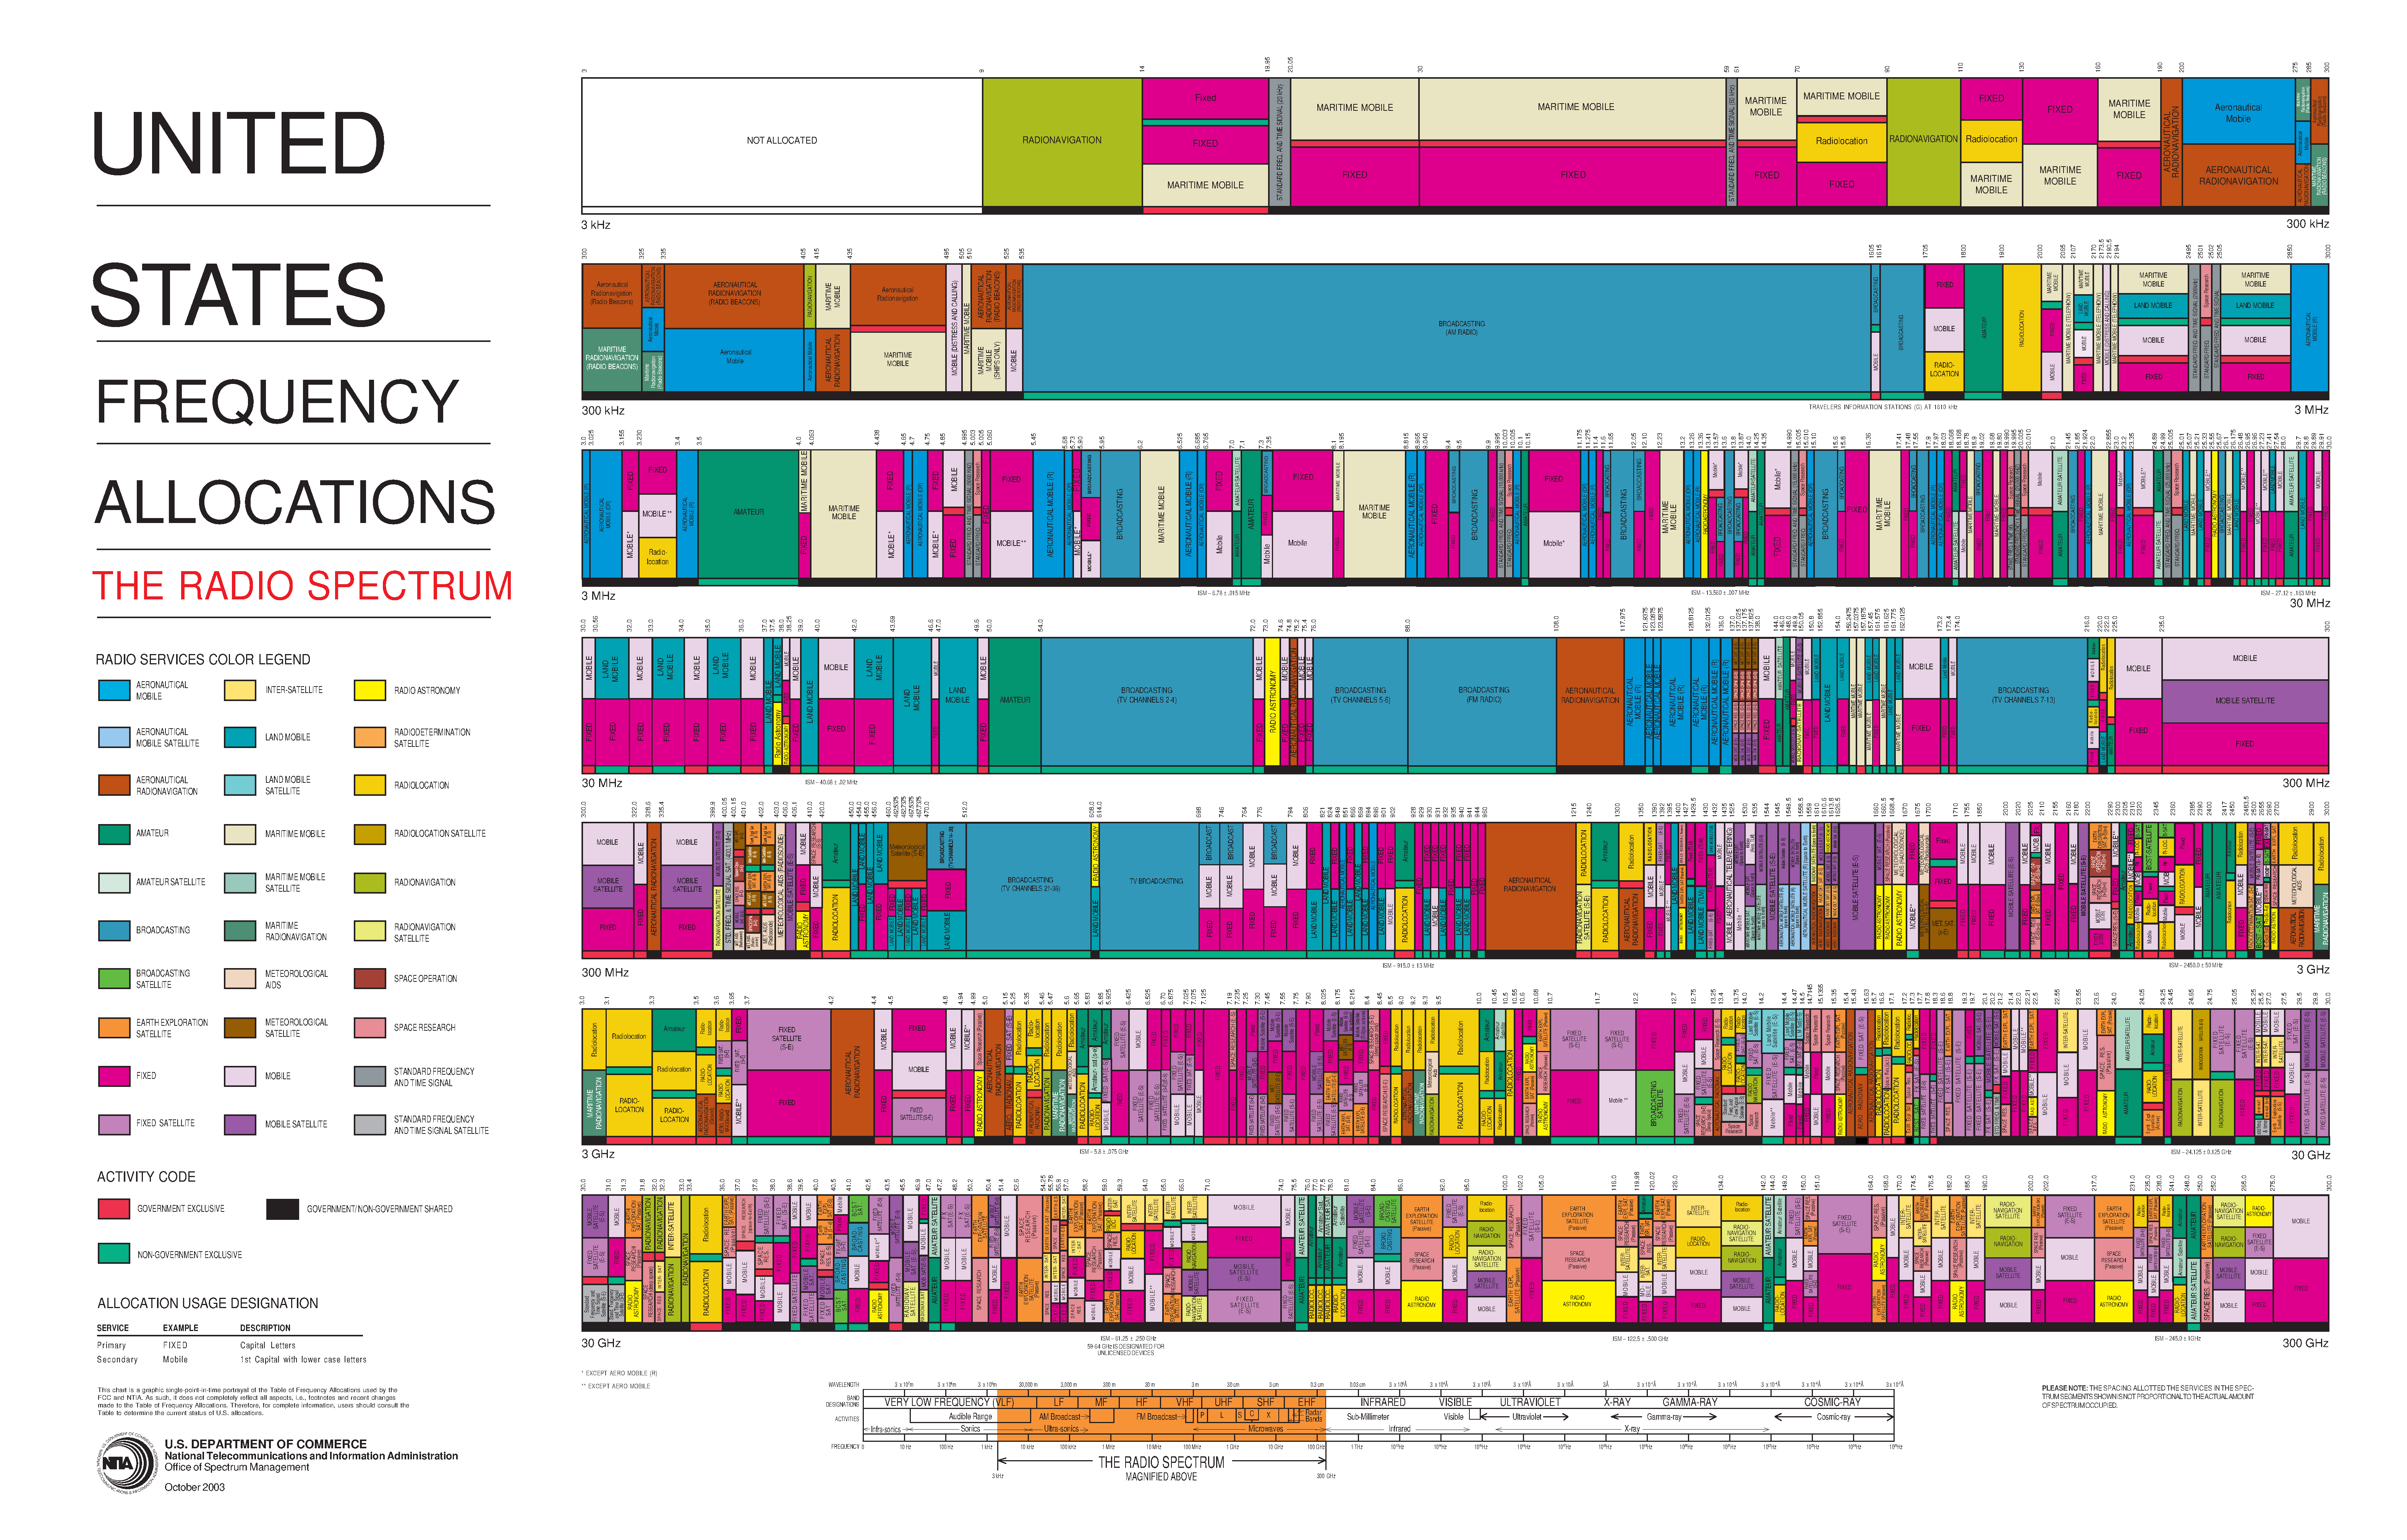
\includegraphics[width=\textwidth]{2003-allochrt.pdf}
\end{center}
\end{frame}

\begin{frame}
\frametitle{Title}
hello world
\end{frame}

\begin{frame}
\frametitle{Title}
hello world
\end{frame}

\begin{frame}
\frametitle{Title}
hello world
\end{frame}

\begin{frame}
\frametitle{Title}
hello world
\end{frame}

\begin{frame}
\frametitle{Title}
hello world
\end{frame}

\begin{frame}
\frametitle{Title}
hello world
\end{frame}

\begin{frame}
\frametitle{Title}
hello world
\end{frame}

\begin{frame}
\frametitle{Title}
hello world
\end{frame}

\begin{frame}
\frametitle{Title}
hello world
\end{frame}

\begin{frame}
\frametitle{Title}
hello world
\end{frame}

\begin{frame}
\frametitle{Title}
hello world
\end{frame}

\begin{frame}
\frametitle{Title}
hello world
\end{frame}

\begin{frame}
\frametitle{Title}
hello world
\end{frame}

\begin{frame}
\frametitle{Title}
hello world
\end{frame}

\begin{frame}
\frametitle{Title}
hello world
\end{frame}

\begin{frame}
\frametitle{Title}
hello world
\end{frame}

\begin{frame}
\frametitle{Title}
hello world
\end{frame}

\begin{frame}
\frametitle{Title}
hello world
\end{frame}

\begin{frame}
\frametitle{Title}
hello world
\end{frame}

\begin{frame}
\frametitle{Title}
hello world
\end{frame}

\begin{frame}
\frametitle{Title}
hello world
\end{frame}

\begin{frame}
\frametitle{Title}
hello world
\end{frame}

\begin{frame}
\frametitle{Title}
hello world
\end{frame}

\begin{frame}
\frametitle{Title}
hello world
\end{frame}

\begin{frame}
\frametitle{Title}
hello world
\end{frame}

\begin{frame}
\frametitle{Title}
hello world
\end{frame}

\begin{frame}
\frametitle{Title}
hello world
\end{frame}

\begin{frame}
\frametitle{Title}
hello world
\end{frame}

\begin{frame}
\frametitle{Title}
hello world
\end{frame}

\begin{frame}
\frametitle{Title}
hello world
\end{frame}

\begin{frame}
\frametitle{Title}
hello world
\end{frame}

\begin{frame}
\frametitle{Title}
hello world
\end{frame}

\begin{frame}
\frametitle{Title}
hello world
\end{frame}

\begin{frame}
\frametitle{Title}
hello world
\end{frame}

\begin{frame}
\frametitle{Title}
hello world
\end{frame}

\begin{frame}
\frametitle{Title}
hello world
\end{frame}

\begin{frame}
\frametitle{Title}
hello world
\end{frame}

\begin{frame}
\frametitle{Title}
hello world
\end{frame}

\begin{frame}
\frametitle{Title}
hello world
\end{frame}

\begin{frame}
\frametitle{Title}
hello world
\end{frame}

\begin{frame}
\frametitle{Title}
hello world
\end{frame}

\begin{frame}
\frametitle{Title}
hello world
\end{frame}

\begin{frame}
\frametitle{Title}
hello world
\end{frame}

\begin{frame}
\frametitle{Title}
hello world
\end{frame}

\begin{frame}
\frametitle{Title}
hello world
\end{frame}

\begin{frame}
\frametitle{Title}
hello world
\end{frame}

\begin{frame}
\frametitle{Title}
hello world
\end{frame}

\begin{frame}
\frametitle{Title}
hello world
\end{frame}

\begin{frame}
\frametitle{Title}
hello world
\end{frame}

\begin{frame}
\frametitle{Title}
hello world
\end{frame}

\begin{frame}
\frametitle{Title}
hello world
\end{frame}

%
%\begin{frame}
%\frametitle{Title}
%hello world
%\end{frame}
%
\end{document}